%to have line numbers
%\RequirePackage{lineno}
\documentclass[10pt, letterpaper]{article}      
\usepackage[margin=.1cm,font=small,labelfont=bf]{caption}[2007/03/09]
%\usepackage{endnotes}
%\let\footnote=\endnote
\usepackage{setspace}
\usepackage{longtable}                        
\usepackage{anysize}                          
\usepackage{natbib}                           
%\bibpunct{(}{)}{,}{a}{,}{,}                   
\bibpunct{(}{)}{,}{a}{}{,}                   
\usepackage{amsmath}
\usepackage[% draft,
pdftex]{graphicx} %draft is a way to exclude figures                
\usepackage{epstopdf}
\usepackage{hyperref}                             % For creating hyperlinks in cross references
\hypersetup{pdfborder={0 0 0.4}} %have nice light boxes on refs

% \usepackage[margins]{trackchanges}

% \note[editor]{The note}
% \annote[editor]{Text to annotate}{The note}
%    \add[editor]{Text to add}
% \remove[editor]{Text to remove}
% \change[editor]{Text to remove}{Text to add}

%TODO make it more standard before submission: \marginsize{2cm}{2cm}{1cm}{1cm}
\marginsize{1cm}{1cm}{.5cm}{.5cm}%{left}{right}{top}{bottom}   
					          % Helps LaTeX put figures where YOU want
 \renewcommand{\topfraction}{1}	                  % 90% of page top can be a float
 \renewcommand{\bottomfraction}{1}	          % 90% of page bottom can be a float
 \renewcommand{\textfraction}{0.0}	          % only 10% of page must to be text

 \usepackage{float}                               %latex will not complain to include float after float

\usepackage[table]{xcolor}                        %for table shading
\definecolor{gray90}{gray}{0.90}
\definecolor{orange}{RGB}{255,128,0}

\renewcommand\arraystretch{.9}                    %for spacing of arrays like tabular

%-------------------- my commands -----------------------------------------
\newenvironment{ig}[1]{
\begin{center}
 %\includegraphics[height=5.0in]{#1} 
 \includegraphics[height=3.3in]{#1} 
\end{center}}

 \newcommand{\cc}[1]{
\hspace{-.13in}$\bullet$\marginpar{\begin{spacing}{.6}\begin{footnotesize}\color{blue}{#1}\end{footnotesize}\end{spacing}}
\hspace{-.13in} }

%-------------------- END my commands -----------------------------------------



%-------------------- extra options -----------------------------------------

%%%%%%%%%%%%%
% footnotes %
%%%%%%%%%%%%%

%\long\def\symbolfootnote[#1]#2{\begingroup% %these can be used to make footnote  nonnumeric asterick, dagger etc
%\def\thefootnote{\fnsymbol{footnote}}\footnote[#1]{#2}\endgroup}	%see: http://help-csli.stanford.edu/tex/latex-footnotes.shtml

%%%%%%%%%%%
% spacing %
%%%%%%%%%%%

% \abovecaptionskip: space above caption
% \belowcaptionskip: space below caption
%\oddsidemargin 0cm
%\evensidemargin 0cm

%%%%%%%%%
% style %
%%%%%%%%%

%\pagestyle{myheadings}         % Option to put page headers
                               % Needed \documentclass[a4paper,twoside]{article}
%\markboth{{\small\it Politics and Life Satisfaction }}
%{{\small\it Adam Okulicz-Kozaryn} }

%\headsep 1.5cm
% \pagestyle{empty}			% no page numbers
% \parindent  15.mm			% indent paragraph by this much
% \parskip     2.mm			% space between paragraphs
% \mathindent 20.mm			% indent math equations by this much

%%%%%%%%%%%%%%%%%%
% extra packages %
%%%%%%%%%%%%%%%%%%

\usepackage{datetime}


\usepackage[latin1]{inputenc}
\usepackage{tikz}
\usetikzlibrary{shapes,arrows,backgrounds}


%\usepackage{color}					% For creating coloured text and background
%\usepackage{float}
\usepackage{subfig}                                     % for combined figures

\renewcommand{\ss}[1]{{\colorbox{blue}{\bf \color{white}{#1}}}}
\newcommand{\ee}[1]{\endnote{\vspace{-.10in}\begin{spacing}{1.0}{\normalsize #1}\end{spacing}\vspace{.20in}}}
\newcommand{\emd}[1]{\ExecuteMetaData[/tmp/tex]{#1}} % grab numbers  from stata

%TODO before submitting comment this out to get 'regular fornt'
\usepackage{sectsty}
\allsectionsfont{\normalfont\sffamily}
\usepackage{sectsty}
\allsectionsfont{\normalfont\sffamily}
\renewcommand\familydefault{\sfdefault}

%\usepackage[margins]{trackchanges}
\usepackage{rotating}
\usepackage{catchfilebetweentags}

\usepackage{abstract}
\renewcommand{\abstractname}{}    % clear the title
\renewcommand{\absnamepos}{empty} % originally center
%-------------------- END extra options -----------------------------------------
\date{{}\today \hspace{.2in}\xxivtime}
\title{  % remember to have Vistula University!!
  Hey! Cities! Leave Them Kids Alone!\footnote{The title paraphrizes Pink
    Floyd's song: \url{https://www.youtube.com/watch?v=qs35t2xFqdU}} \\
  \Large{(Urban Adolescents Have Lower Life Satisfaction and Eudamonia)} % than rural ones %(urban unhappiness is common in adolescents)
}
\author{
% Adam Okulicz-Kozaryn\thanks{EMAIL: adam.okulicz.kozaryn@gmail.com
%   \hfill I thank XXX.  All mistakes are mine.} \\
% {\small Rutgers - Camden  % and Vistula University
% }
}

\begin{document}

%%\setpagewiselinenumbers
%\modulolinenumbers[1]
%\linenumbers

\bibliographystyle{/home/aok/papers/root/tex/ecta}
\maketitle
\vspace{-.4in}
\begin{center}

\end{center}


\begin{abstract}
\noindent strong effects! on the whole, about 0.5 on 1-10 scale, and for some
countries close to 1! Not just cognitive life satisfaction, but also rarely
studied Eudamonia. By studying adolescents, we are able to refute self-sorting
counterarguments, i.e., that cities do not produce unhappiness but unhappy
people move to cities--adolescents in general do not move, but are born into a
place. 
\end{abstract}
\vspace{.15in} 
\noindent{\sc %XXX TODO add to ebib as keyword PAPER-CODE-NAME and tag with ebib keywords 
} 
\vspace{.25in} 

\begin{spacing}{1.4} %TODO MAYBE before submission can make it like 2.0
\rowcolors{1}{white}{gray90}

%  instead \ExecuteMetaData[../out/tex]{ginipov} do \emd{ginipov}

% \begin{figure}[H]
%  \includegraphics[height=3in]{../out/gov_res_trust.pdf}\centering\label{gov_res_trust}
% \caption{woo}
% \end{figure}


%TODO !!!! have input here aok_var_des

Happiness may not be the ultimate goal for adults (but duty, service, doing the
right thing, etc), but what else we want for kids if not happiness. And what
else kids want themselves if not happiness. 
Findings should be of interest to policymakers, administrators, schools,
parents--to achieve greater happiness for the kids, kids should experience more
urbanity or rurality?

We know that adults tend to be less happy in cities across the world (except in
the poorest nations such as Sub-Saharan Africa) \citep{aok21}. But we do not
know about the children. 

\section*{Theory and Mechanisms of Urban Unhappiness}

% rephraze copied from swbUrbRurPsid
 Genes determine about half of SWB
 \citep{schnittker08,lykken96t,brooksGenetic}.
 %
 Humans have not
evolved for city life among thousands of people densely packed together in an
artificial setting, a city. Some animals such as ants or bees may thrive at a
high density, but human nature is unlike that of bees: by one estimate we're 90\% chimp and only 10\% bee  \citep{haidt12B}.
For over 95\% of human evolutionary history there were no cities--hunters-gatherers lived in bands of 50-80 \citep{maryanski92}. 
%Humans have evolved to prefer and be happy in nature,  open space
%there was that citation that i have recently seen but forgot where that that
%humans evolved to prefer nature--those who prefered it and were in harmony with
%it were more likely to survive etc


Ingroup preference or homophily (``love of the same'') theory
  states 
that a  human has a preference for other humans like her \citep{mcpherson01,tajfel82,tajfel71,smelser99,putnam07,christakis09f}. % , and outgroups contain dissimilar persons.
 A defining
feature of a city is heterogeneity or diversity \citep{wirth38}, which
accordingly produces: 
 mistrust, uneasiness, conflict, and misanthropy
 \citep{milgram70,thrift05,amin06}.\footnote{
 Yet, on the other hand, in a city there can be community, a neighborhood
village, that at least in some ways can simulate a more natural habitat for a
human \citep{fischer95,fischer75,jacobs93}.}

Livability theory \citep{veenhoven95,veenhoven14b,veenhoven00b} states that
humans, just as other animals, have needs (such as those on Maslow hierarchy of
needs \citep{maslow87}), and if those needs are satisfied, then conditions are
livable and happiness follows. As opposed to evolution and homophily
predicting urban unhappiness, it is unclear what livability theory
 predicts regarding urbanism. Some aspects of urbanism may
 improve livability, and hence, happiness.
  %
 Cities have multiple benefits  \citep{meyer13,florida08,glaeser11,osullivan09}, notably jobs and amenities that improve livability and
 happiness. But cities also do have multiple disamenities such as more congestion, crime,
   infectious  disease spread, air, noise, and light pollutions
   \citep{bettencourt10b,bettencourt07,meyer13,aokCityBook15}.\footnote{Measuring
     it with happiness yardstick,  city disadvantages outweigh city
     advantages--cities are less happy (at least in the developed world)
     \citep{aok21}.} 
 %
   And those disamenities may especially affect adolescents. Urban
 crime (and bullying) is perhaps more of a problem for adolescents (especially
 females) than for adults who may be better able to insulate themselves from
 it\footnote{An adult would spend much time at work, home, or in a
   car, which are relatively crime free. An adolescent is arguably less able to
   insulate herself from neighborhood and peers, which are often infested with
   crime in large cities. It needs to be remebered that crime is a a city
   feature--all large cities have large crime problem--crime  does increase
   extremely consistently with city size \cite{blissCL_nov4_14,bettencourt13,bettencourt10,bettencourt10b,bettencourt07}.}
 and cope with it. Clearly, by definition, adults have better coping mechanisms
 than more fragile adolescents--coping increases with age \citep{leipold2019coping}. 

 It has been theoretized already a century ago that urbanism has a negative
 effect on human brains / neural processing \citep{simmel03}, and it has been
 recently confirmed by neuroscience, including that even growing up in a city has
 lasting negative effects later in life \citep{lederbogen11}. Again adolescents
 are arguably more at risk than adults. 
   
   Multiple Discrepancies Theory (MDT) \citep{michalos85,michalos14c} states that
happiness is relative and a result of multiple comparisons. Visual and social comparisons are more likely in
urban areas as there are more people and more stimuli. And there is some
evidence that humans tend to make upwards comparisons \citep{frey02s} thus
ending up relatively deprived \citep[e.g.,][]{luttmer05,frank12}. 
 %
 Adolescents, like adults, are likely to want to keep up with Joneses, just in
slightly different ways, e.g., clothing, jewelry, parties, cars--see some
examples in \citet{frank12}.
 %
 And there are usual mechanisms, same as for adults. The more city, the less
nature \cite{aokCityBook15} and nature is the key for human flourishing, maybe even more so for the children and
adolescents who actually have time to experience it \citep{pretty12}. Cities are
 the most polluted places (although they pollute least per capita) 
 \cite{meyer13}, and not just air, but also light and noise polluted. Pollutions,
 of course, kill happiness \cite{signoretta19,poonCL18jan29,leeTT16feb13,metcalfeCL16jun10,weinhold12,rehdanz08,welsch05,york03} 
 Materialism and consumerism (and unethical behavior) are as prevalent as pollutions but arguably more
 overlooked and more urban
 \citep[e.g.,][]{aok-sizeFetish17,okulicz2022materialism,morris21,wirth38} and
 materialism and consumerism are likely to result in unhappiness especially if
 they are on stuff and not experience and at a cost of human needs such as social connection
 \citep[e.g.,][]{frank12,leonard10,vanboven05,burroughs02,dumludag21} (but see
 \citet{wu20,wang17,brown19,brown17}). And the smaller the place, the more
 homegeneity, the more trust and wellebing \citep{putnam07,aok22,herbst14,vogt07}.


Studying urban-rural happiness gradient in kids/adolescents has an advantage
over adults. Some argue that there may be self sorting of unhappy adults into
cities, i.e. it is not that cities make people unhappy, but that unhappy people
move to cities. For instance, ``Veenhoven (1994) argues that cities attract
those already dissatisfied with their life in rural areas, and hence there could
be an excess of unhappy/unsatisfied people in cities. For him, cities do not
make unhappy people but attract them.''\citep[cited in
][]{ebshoy24}. Children/adolescents do not self-sort or move into areas, they
are born into areas. The issue was somewhat addressed in \citet{aok20}, which
utilized the US GSS item ``Which of the categories on this
card comes closest to the type of place you were living in when you were 16
years old?''
 Here instead of asking adults to recall adolescence, we study actual
adolescents, 15yo, and not just in the US, but across the world. 


\section*{Happiness in Kids}

TODO: write sth about happness in kids; btw looks like they used normal happiness question; not smileys


\section*{Data}

We use 2018 PISA (Programme for International Student Assessment) from
\url{https://www.oecd.org/pisa/data/2018database/}. Adolescents are 15 (several percent upto 16.3).

PISA is a large dataset for 142 countries with $>.5m$ observations. And it has a
wellbeing module with dozens of SWB items. At the same time it is not widely
used in the field--indeed we would like advertise PISA data for happiness and in general social indicators
research. We do not have any relationship with OECD or PISA and no conflict of
interest. 

Urbanicity is recorded in  School questionnaire administered to school
principals:

Which of the following definitions best describes the community in which your school is located?
\begin{itemize}
\item A village, hamlet or rural area (fewer than 3 000 people)
\item A small town (3 000 to about 15 000 people)
\item A town (15 000 to about 100 000 people)
\item A city (100000 to about 1 000 000 people)
\item A large city (with over 1 000 000 people). This is an advantage over
  widely used World Values Survey, where the top cutoff is only .5m \cite{deb23,ebshoy24}.
\end{itemize}

A nice feature of PISA data is that urbanicity is missing for only 5.5 percent of
observations. 

There are limitations. There are no measures of siblings and grandparents.  
We do not see a good health variable--exisiting ones are
missing for vast majroity. Health is of course a key happiness predictor, but
arguably less imoportant for kids as they are healthier than adults, and as age
is constant there is less variability in health, too. 

PISA has usual life satisfaction 0-10 measure: ``Overall, how satisfied are you
with your life as a whole these days?'' 

PISA 2018 defines meaning in life as the extent to which 15-year-olds
comprehend, make sense of, or find significance in their lives
\citep{pisa18}. PISA 2018 asked students whether they agree or disagree (
"strongly disagree", "disagree", "agree", "strongly agree") with the following
statements: "My life has clear meaning or purpose"; "I have discovered a
satisfactory meaning in life"; and "I have a clear sense of what gives meaning
to my life". These statements were combined to create the index of meaning in
life

A big happiness killer of the youth is social media
\cite{twengeATL17sep,twenge14}.
 %
We control for internet use, and we do  have specific measures how used, eg we
 measure social media use.  We also measure out of school usage and useage ``for
 fun''--see table \ref{var_des} for all variables definitions. 


 
\input{varDes.tex} 

\section*{Results}

%meh have plenty of tables
% \begin{figure}[H]
%  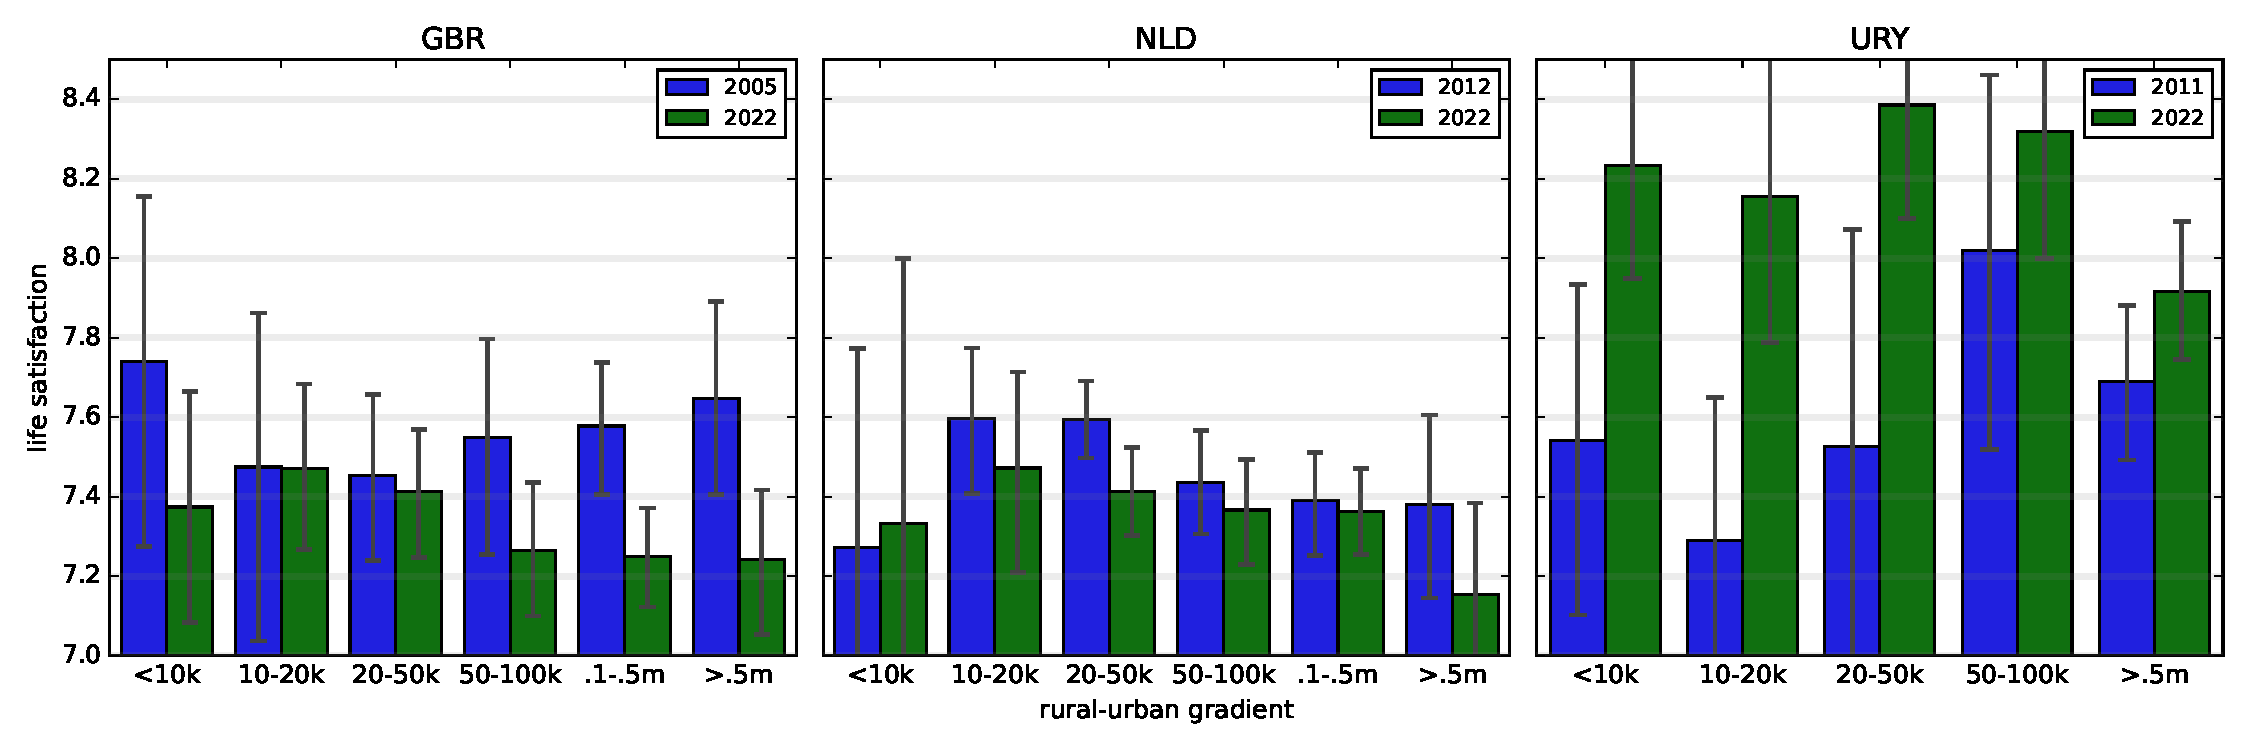
\includegraphics[height=3in]{bar.pdf}\centering\label{bar}
% \caption{Mean of life satisfaction and eudamonia by urbanicity.}
% \end{figure}

 It needs to be remembered
that ecological variables have small effects on SWB as
 expected--most SWB is explained by genes \citep{schnittker08} and person level
 predictors \citep{veenhoven14b}). % . Still, the leading social scientists
 % such as Amartya Sen and Ed Diener advocate use of SWB for
 % public policy \citep{stiglitz09al,diener09}.
 %
 %
 %
 %
  The effect of urbanicity is quite large about .5 on 0-10 SWB scale.
 %  
 Regressions of life satisfaction on urbanicity are shown in table \ref{regA}.\footnote{We use a standard OLS regression with robust standard errors.  We treat the 10-step
happiness variable as continuous. Ordinal happiness can be treated as a
continuous variable \citep{carbonell04}.
%                                                                                                                  
OLS has become the default method in happiness research
\citep{blanchflower11}. Theoretically, while there is still debate about the
cardinality of SWB, there are strong arguments to treat it as a cardinal
variable \citep{ng96,ng97}.
}
 In a1-a3\footnote{Not
in a4 controling for country dummies.} there is a big
difference between the largest cities (gt1m) and smaller areas just like for
adults \citep{aok-ls_fisher16}. But interestingly, not necessarily like adults,
there is also a large gap between lt3k and 3-15k, again especially in models
a1-a3, perhaps in the open country (lt3k) there are best outdoor play opportunities for
the kids.

As in adults \citep{aok21}, addition of income/wealth makes results
stronger--income/wealth confounds with urbanicity.
 %
In full model, a4, effect sizes are large: beta (fully standardized; not shown) for
gt1m is 65 percent of wealth.
 %
 In a4m and a4f we split by gender--interestingly city penaly is higher for
female perhaps because females wellbeing is more affected by urban crime. 
 %
 Model a5  adds the 4 internet use variables in  (we postpone it to
the last model as the internet variables cut the sample size by about 200k),
results are similar\footnote{Actually interent use has very low correlation
  with urbanicity--see online appendix for details. It probably has been the case
  that internet was more of an urban phenomenon, but in an era of
  smartphones--they are ubiquitious throught degrees of urbanness and
  development levels.}
 %
 %arthur
Could it be that children in smaller places don't need as much material wealth
to be happy because they have other non-costly options for entertainment. We
 will test this by interacting the family wealth variable with the urban/rural
categories to see if the effect of material wealth on life satisfaction differs
according to place (hopefully having a smaller effect on happiness in smaller
places). And indeed it is the case in model a6, but then when adding country
dummies the effect goes away in a7. 
% Finally models a6 and a7 add interactions of urbanicity with wealth, while
%  significant in a6, the interactions lose significance when controling for
%  country dummies in a7. 


\begin{table}[H]\centering\caption{OLS regressions of life satisfaction.} \label{regA} \begin{scriptsize} \begin{tabular}{p{1.6in}p{.5in}p{.5in}p{.5in}p{.5in}|p{.5in}p{.5in}|p{.5in}|p{.5in}p{.5in}p{.5 in}p{.5in}p{.5 in}}\hline                     &   $<.5m$   &     $>.5m$   &   $<.5m$   &     $>.5m$   &   URYrurTow   &     URYcity   \\
2022                &       -0.21** &       -0.41** &       -0.12** &       -0.23   &        0.75***&        0.23+  \\
constant            &        7.54***&        7.65***&        7.50***&        7.38***&        7.54***&        7.69***\\
N                   &        3111   &         521   &        3572   &         373   &        1154   &         836   \\
 \hline\multicolumn{4}{l}{*p$<$0.05 **p$<$0.01 ***p$<$0.001} \end{tabular}\end{scriptsize}\end{table}




\begin{spacing}{.9} \begin{table}[H]\centering   \begin{scriptsize} \begin{tabular}{p{.5in}p{.5in}p{.5in}p{.5in}p{.5in}p{.5in}p{.5in}p{.5in}p{.5in}p{.5in}p{.5
                                                                      in}p{.5in}p{.5
                                                                      in}}\hline
                                                                      \input{../out/a4cou.tex}
                                                                      \hline *
                                                                      p$<$0.05,
                                                                      $+$
                                                                      p$<$0.1;
                                                                      robust std
                                                                      err \end{tabular}\end{scriptsize}\caption{\label{a4cou}OLS
                                                                    regressions
                                                                    of life satisfaction on
                                                                    place size
                                                                    for each
                                                                    country
                                                                    separately
                                                                    includiOBng
                                                                    covariates
                                                                    from a4 (not
                                                                    shown). Only
                                                                  LBN and HUN
                                                                  marginally
                                                                  happier in
                                                                  cities lt1m
                                                           }\end{table} \end{spacing}


Results with sampling weights in appendix are similar.
                                                       






\subsection{Eudamonia}

We turn to eudamonia, a rarely studied type of SWB. 
 %
 In table \ref{regB} different from life satisfaction, biggest hit from lt3k to 3-15k in b1-b3, and in b4
controllig for countruy dummies, there is rather a smooth gradient in b4f and
b4m--females lose  abot 2x more eudamonia than males going up on urbanicity.


\begin{table}[H]\centering\caption{OLS regressions of Eudamonia.} \label{regB} \begin{scriptsize} \begin{tabular}{p{1.6in}p{.5in}p{.5in}p{.5in}p{.5in}|p{.5in}p{.5in}|p{.5in}|p{.5in}p{.5in}p{.5 in}p{.5in}p{.5 in}}\hline                     &   $<.5m$   &     $>.5m$   &   $<.5m$   &     $>.5m$   &   URYrurTow   &     URYcity   \\
2022                &       -0.18*  &       -0.39+  &       -0.20***&       -0.45** &        0.42***&        0.21   \\
income              &        0.09***&        0.01   &        0.06***&        0.14***&        0.07*  &        0.13***\\
age                 &       -0.03*  &       -0.08** &       -0.02+  &       -0.06+  &        0.00   &       -0.06** \\
age2                &        0.00** &        0.00** &        0.00** &        0.00*  &       -0.00   &        0.00** \\
male                &       -0.18** &       -0.13   &       -0.11*  &       -0.27+  &        0.06   &        0.19   \\
married or living together as married&        0.53***&        0.74***&        0.44***&        0.23   &        0.46** &        0.06   \\
divorced/separated/widowed&        0.07   &        0.15   &       -0.11   &       -0.14   &       -0.37+  &       -0.19   \\
autonomy            &       -0.11*  &       -0.07   &       -0.11** &       -0.01   &       -0.06   &        0.06   \\
freedom             &        0.44***&        0.42***&        0.35***&        0.43***&        0.43***&        0.36***\\
trust               &        0.12+  &        0.42** &        0.43***&        0.28+  &       -0.05   &        0.10   \\
postmaterialist     &       -0.05   &       -0.18   &       -0.11*  &        0.14   &       -0.02   &        0.15   \\
god important       &        0.01   &        0.05*  &        0.02*  &       -0.01   &        0.05** &        0.06** \\
constant            &        4.08***&        5.95***&        4.59***&        4.80***&        3.47***&        4.58***\\
N                   &        1985   &         309   &        2283   &         237   &         736   &         579   \\
 \hline\multicolumn{4}{l}{*p$<$0.05 **p$<$0.01 ***p$<$0.001} \end{tabular}\end{scriptsize}\end{table}

And like with life satisfaction in a5 controling for internet use does not change gt1m
coefficent significantly in b5.
Urban penalty of about .1-.15 is substantial as eduamonia ranges -2.1 to  1.7
with IQR -.6 to .8. In b7 unexpectedly wealth matters less in large cities. 


In table \ref{b4cou} urban eudamonia penalty is less clear than life
satisfaction--while most countries do have urban penalty, there is a handful
with urban eudamonic premium. 


\begin{spacing}{.9} \begin{table}[H]\centering   \begin{scriptsize} \begin{tabular}{p{.5in}p{.5in}p{.5in}p{.5in}p{.5in}p{.5in}p{.5in}p{.5in}p{.5in}p{.5in}p{.5
                                                                      in}p{.5in}p{.5
                                                                      in}}\hline
                                                                      \input{../out/b4cou.tex}
                                                                      \hline *
                                                                      p$<$0.05,
                                                                      $+$
                                                                      p$<$0.1;
                                                                      robust std
                                                                      err \end{tabular}\end{scriptsize}\caption{\label{b4cou}OLS
                                                                    regressions
                                                                    of Eudamonia on
                                                                    place size
                                                                    for each
                                                                    country
                                                                    separately
                                                                    including
                                                                    covariates
                                                                    from b4 (not
                                                                    shown). Most
                                                                    countries
                                                                    eudamoinc
                                                                    urban
                                                                    penalty, but
                                                                    a
                                                                    handful of
                                                                    countries
                                                                    have premium
                                                           }\end{table} \end{spacing}



Results with sampling weights in appendix are weaker.

\section*{Conclusion and discussion}


Findings should be of interest to policymakers, administrators, schools,  parents. To achieve greater happiness for the kids, kids should enjoy more rurality.


%adam
Happiness may not be the ultimate goal for adults (eg duty, service, doing the right thing), but what else we want for kids if not happiness.
 Rurality arguably is a more fertile ground for  spontaneity and freedom--in
 rural can just go out there and hang out and have fun, fewer rules and
 restrictions; city can weigh down especially on kids and elderly with its
 setup, rules and complexity. City is really made for working age adults to do
 work and consume. Kids and elderly are neither productive for jobs nor fit for
 many city amenities like airports, universities, etc. (but are for others like
 entertainment, hospitals etc). 
%
We have cities and density to produce stuff \citep{osullivan09}, like in Engels'
Manchester, where a capitalist crammed factory workers to produce.\footnote{\begin{quote}
In a rather deep hole, in a curve
of the Medlock and surrounded on all four sides by tall factories and high embankments, covered with
buildings, stand two groups of about two hundred cottages, built chiefly back to back, in which live about four
thousand human beings, most of them Irish. The cottages are old, dirty, and of the smallest sort, the streets
uneven, fallen into ruts and in part without drains or pavement; masses of refuse, offal and sickening filth lie
among standing pools in all directions; the atmosphere is poisoned by the effluvia from these, and laden and
darkened by the smoke of a dozen tall factory chimneys. A horde of ragged women and children swarm about
here, as filthy as the swine that thrive upon the garbage heaps and in the puddles. In short, the whole rookery
furnishes such a hateful and repulsive spectacle as can hardly be equalled in the worst court on the Irk. The
race that lives in these ruinous cottages, behind broken windows, mended with oilskin, sprung doors, and
rotten door-posts, or in dark, wet cellars, in measureless filth and stench, in this atmosphere penned in as if
with a purpose, this race must really have reached the lowest stage of
humanity. \citep{engels87}
\end{quote}
} Now factories are largely gone to China, and what was left of productive city
was office. But COVID shook that up too. So now really the main thing is amenities like airports, hospitals, etc. 

Wealth does matter a lot in the city, it's totally different life at top and
bottom in the city. Still when accounting for country dummies, we do not find
differential positive effect of wealth in cities on life satisfaction, and if
anything negative with eudamonia. 

 % rubia
We would  like to take into account granparents and siblings, but we do not have
such measures in 2018 PISA. % also look into the caretakers and extended family (grandparents).
 In cities, most people tend to leave with their nuclear family, far away from
 relatives and both parents usually work leaving their kids at day care or with
 nannies who arent related to them. Parents spend less time with their kids as a
 result. Whereas in smaller places, its possible that the kids have more contact
 and spend more time with at least one of the parents (main caregiver) or with
 grandparents and other extended relatives. 
 Also future research should be  controlling for number of siblings. Kids having other kids around to interact and play with might be a factor too.
 Finally, arguably after the pandemic adolescents in cities became even more unhappy just as adults did
\textbf{<<blind for peer-review>>}. 

                                                       
% %table centered on decimal points:)
% \begin{table}[H]\centering\footnotesize
% \caption{\label{freq_im_god} importance of God}
% \begin{tabular} {@{} lrrrr @{}}   \hline 
% Item& Number & Per cent   \\ \hline
% 1(not at all)&    9,285&  9\\
% 2&    3,555&        3\\
% 3&    3,937&        4\\
% 4&    2,888&        3\\
% 5&    7,519&        7\\
% 6&    5,175&        5\\
% 7&    6,050&        6\\
% 8&    8,067&        8\\
% 9&    8,463&        8\\
% 10&   52,385&       49\\
% Total&  107,324&      100\\ \hline
% \end{tabular}\end{table}


% % Define block styles
% \tikzstyle{block} = [rectangle, draw, fill=black!20, 
%     text width=10em, text centered, rounded corners, minimum height=4em]
% \tikzstyle{b} = [rectangle, draw,  
%     text width=6em, text centered, rounded corners, minimum height=4em]
% \tikzstyle{line} = [draw, -latex']
% \tikzstyle{cloud} = [draw, ellipse,fill=black!20, node distance = 5cm,
%     minimum height=2em]
    
% \begin{tikzpicture}[node distance = 2cm, auto]
%     % Place nodes
%     \node [block] (lib) {liberalism, egalitarianism, welfare};
%     \node [block, below of=lib] (con) {conservatism, competition, individualism};
%     \node [cloud, right of=con] (ls) {well-being};
%     \node [block, below of=ls] (cul) {genes, culture};
%     \node [b, left of =lib, node distance = 4cm] (c) {country-level};
%     \node [b, left of =con,  node distance = 4cm] (c) {person-level};
%     % Draw edges
%     \path [line] (lib) -- (ls);
%     \path [line] (con) -- (ls);
%     \path [line,dashed] (cul) -- (ls);
% \end{tikzpicture}


%PUT THIS NOTE, polish and put to /root/author_what_data --ALWAYS
%stick here stuff as i run it!!! maybe comment out later...


% TODO: have separate som-r.tex as opposed to having it below; and in paper say
% see supplemetary material as opposed to see appendix!

%\newpage
%\theendnotes
\bibliography{/home/aok/papers/root/tex/ebib.bib,/home/aok/papers/root/old/2022/swbUrbRurPsid/tex/swbUrbRurPsid.bib,pisa.bib}


 \section*{\Huge ONLINE APPENDIX}
 \textbf{[note: this section will NOT be a part of the final version of
   the manuscript, but will be available online instead]} %hence everything below
                                 %is organized byu section, not subsection
% !!!
% have most of the stuff outputted to online appendix:)--start with that and then
% select stuff to paper--have brief narrative describng patterns in online app too
% !!!

% \section*{Variables' definitions, coding, and distributions}
% \label{app_var_des}



\begin{spacing}{.9} \begin{table}[H]\centering   \begin{scriptsize} \begin{tabular}{p{.5in}p{.5in}p{.5in}p{.5in}p{.5in}p{.5in}p{.5in}p{.5in}p{.5in}p{.5in}p{.5
                                                                      in}p{.5in}p{.5
                                                                      in}}\hline
                                                                      \input{../out/a1.tex}
                                                                      \hline *
                                                                      p$<$0.05,
                                                                      $+$
                                                                      p$<$0.1;
                                                                      robust std
                                                                      err \end{tabular}\end{scriptsize}\caption{\label{d1}OLS
                                                                    regressions
                                                                    of SWB on
                                                                    place size
                                                                    only
                                                                    (bivariate; a1)
                                                                    for each
                                                                    country
                                                                    separately. 
                                                                  }\end{table} \end{spacing}


\section{internet use}

Urbanicity has very low positive correlation with internet use

\begin{spacing}{.5}
\begin{scriptsize}
\begin{verbatim}
. d city int*

Variable      Storage   Display    Value
    name         type    format    label      Variable label
-------------------------------------------------------------------------------
city            byte    %9.0g      city       RECODE of SC001Q01TA (Which of
                                                the following definitions best
                                                describes the comm
intWday         byte    %2.0f      labels341
                                              During a typical weekday, for how
                                                long do you use the Internet
                                                outside of school
intWend         byte    %2.0f      labels342
                                              On a typical weekend day, for how
                                                long do you use the Internet
                                                outside of school
intSN           byte    %2.0f      labels374
                                              Use digital devices outside of
                                                school: Participating in Social
                                                Networks (e.g. <F
intFun          byte    %2.0f      labels376
                                              Use digital devices outside of
                                                school: Browsing the Internet
                                                for fun (such as wa


. pwcorr city int*

             |     city  intWday  intWend    intSN   intFun
-------------+---------------------------------------------
        city |   1.0000 
     intWday |   0.0488   1.0000 
     intWend |   0.0720   0.7251   1.0000 
       intSN |   0.0569   0.2594   0.2792   1.0000 
      intFun |   0.0866   0.3066   0.3479   0.5249   1.0000 
\end{verbatim}
\end{scriptsize}
\end{spacing}{.9}

Using some internet is good for an adolescent, but using a lot on the weekend is bad


\begin{spacing}{.5}
\begin{scriptsize}
\begin{verbatim}
reg ls i.city wealth fem faEd i.intWday i.intWend, robust

Linear regression                               Number of obs     =    266,770
                                                F(19, 266750)     =     340.73
                                                Prob > F          =     0.0000
                                                R-squared         =     0.0238
                                                Root MSE          =     2.5032

------------------------------------------------------------------------------
             |               Robust
          ls | Coefficient  std. err.      t    P>|t|     [95% conf. interval]
-------------+----------------------------------------------------------------
        city |
      3-15k  |  -.4296694   .0196451   -21.87   0.000    -.4681732   -.3911656
    15-100k  |  -.4853962   .0185923   -26.11   0.000    -.5218366   -.4489557
    100k-1m  |  -.5295389   .0186871   -28.34   0.000    -.5661651   -.4929126
       gt1m  |  -.7087667   .0212434   -33.36   0.000    -.7504032   -.6671301
             |
      wealth |    .058285   .0053595    10.87   0.000     .0477805    .0687896
         fem |  -.4855582   .0097124   -49.99   0.000    -.5045942   -.4665223
        faEd |  -.0238479   .0051004    -4.68   0.000    -.0338445   -.0138513
             |
     intWday |
1-30 minu..  |   .1687749   .0381252     4.43   0.000     .0940505    .2434993
31-60 min..  |   .1174412   .0369693     3.18   0.001     .0449823    .1899001
Between 1..  |   .0837295   .0347786     2.41   0.016     .0155643    .1518946
Between 2..  |  -.0017767   .0345739    -0.05   0.959    -.0695406    .0659872
Between 4..  |  -.0369376   .0357303    -1.03   0.301    -.1069681    .0330928
More than..  |   .0083298   .0365747     0.23   0.820    -.0633557    .0800153
             |
     intWend |
1-30 minu..  |    .241415    .046509     5.19   0.000     .1502586    .3325714
31-60 min..  |    .296678   .0448001     6.62   0.000     .2088711     .384485
Between 1..  |   .2990314    .042022     7.12   0.000     .2166694    .3813934
Between 2..  |      .1492   .0414603     3.60   0.000     .0679389     .230461
Between 4..  |  -.0009641   .0418857    -0.02   0.982     -.083059    .0811307
More than..  |  -.2383889   .0423359    -5.63   0.000    -.3213662   -.1554117
             |
       _cons |   7.966607   .0429739   185.38   0.000     7.882379    8.050834
------------------------------------------------------------------------------
\end{verbatim}
\end{scriptsize}
\end{spacing}{.9}



And below another robustness check, using clustered std err on school and school
level covariates--results similar
\begin{spacing}{.5}
\begin{scriptsize}
\begin{verbatim}

. d STRATIO SCHLTYPE CLSIZE EDUSHORT STAFFSHORT STUBEHA TEACHBEHA 

Variable      Storage   Display    Value
    name         type    format    label      Variable label
------------------------------------------------------------------------------
STRATIO         double  %10.0g                Student-Teacher ratio
SCHLTYPE        byte    %10.0g                School Ownership
CLSIZE          byte    %10.0g                Class Size
EDUSHORT        double  %10.0g                Shortage of educational material
                                                (WLE)
STAFFSHORT      double  %10.0g                Shortage of educational staff
                                                (WLE)
STUBEHA         double  %10.0g                Student behaviour hindering
                                                learning (WLE)
TEACHBEHA       double  %10.0g                Teacher behaviour hindering
                                                learning (WLE)


. reg ls i.city wealth i.gender faEd i.Region STRATIO SCHLTYPE CLSIZE EDUSHORT
>  STAFFSHORT STUBEHA TEACHBEHA , robust cluster(CNTSCHID)

Linear regression                               Number of obs     =    389,098
                                                F(131, 15010)     =     129.21
                                                Prob > F          =     0.0000
                                                R-squared         =     0.0686
                                                Root MSE          =      2.488

                          (Std. err. adjusted for 15,011 clusters in CNTSCHID)
------------------------------------------------------------------------------
             |               Robust
          ls | Coefficient  std. err.      t    P>|t|     [95% conf. interval]
-------------+----------------------------------------------------------------
        city |
      3-15k  |      -0.19       0.02    -8.07    0.00        -0.24       -0.14
    15-100k  |      -0.26       0.02   -11.18    0.00        -0.31       -0.22
    100k-1m  |      -0.41       0.02   -16.91    0.00        -0.45       -0.36
       gt1m  |      -0.44       0.03   -16.02    0.00        -0.49       -0.38
             |
      wealth |       0.21       0.01    38.32    0.00         0.20        0.22
             |
      gender |
       Male  |       0.40       0.01    42.56    0.00         0.38        0.42
        faEd |      -0.02       0.00    -5.15    0.00        -0.03       -0.01
             |
      Region | -----COUNTRY DUMMIES OMITTED HERE---------
             |
     STRATIO |       0.00       0.00     0.71    0.48        -0.00        0.00
    SCHLTYPE |       0.06       0.01     5.75    0.00         0.04        0.09
      CLSIZE |       0.00       0.00     2.39    0.02         0.00        0.00
    EDUSHORT |       0.01       0.01     2.07    0.04         0.00        0.03
  STAFFSHORT |      -0.01       0.01    -1.07    0.29        -0.02        0.01
     STUBEHA |       0.01       0.01     1.15    0.25        -0.01        0.02
   TEACHBEHA |      -0.02       0.01    -2.34    0.02        -0.03       -0.00
       _cons |       8.66       0.07   117.75    0.00         8.52        8.81
------------------------------------------------------------------------------




\end{verbatim}
\end{scriptsize}
\end{spacing}{.9}

Finally sampling weights--results similar for life satisfaction, but weaker for
eudamonia. Also see
\url{https://www.statalist.org/forums/forum/general-stata-discussion/general/1435058-should-i-apply-weights-when-i-use-the-tabulate-command-oecd-pisa-analysis}
and \url{https://largescaleassessmentsineducation.springeropen.com/articles/10.1186/s40536-021-00099-0}

\begin{spacing}{.5}
\begin{scriptsize}
\begin{verbatim}

. reg ls i.city, robust  //it is huuuge yay!

Linear regression                               Number of obs     =    471,551
                                                F(4, 471546)      =     398.44
                                                Prob > F          =     0.0000
                                                R-squared         =     0.0034
                                                Root MSE          =     2.5877

------------------------------------------------------------------------------
             |               Robust
          ls | Coefficient  std. err.      t    P>|t|     [95% conf. interval]
-------------+----------------------------------------------------------------
        city |
      3-15k  |      -0.34       0.01   -23.16    0.00        -0.37       -0.32
    15-100k  |      -0.37       0.01   -26.19    0.00        -0.40       -0.34
    100k-1m  |      -0.44       0.01   -30.78    0.00        -0.47       -0.41
       gt1m  |      -0.61       0.02   -38.86    0.00        -0.64       -0.58
             |
       _cons |       7.63       0.01   624.06    0.00         7.61        7.66
------------------------------------------------------------------------------

. 
end of do-file

. do "/tmp/SD17808.000000"

. reg ls i.city [pw=W_FSTUWT], robust 
(sum of wgt is 24,137,093.50498)

Linear regression                               Number of obs     =    471,551
                                                F(4, 471546)      =     107.54
                                                Prob > F          =     0.0000
                                                R-squared         =     0.0060
                                                Root MSE          =      2.611

------------------------------------------------------------------------------
             |               Robust
          ls | Coefficient  std. err.      t    P>|t|     [95% conf. interval]
-------------+----------------------------------------------------------------
        city |
      3-15k  |      -0.31       0.04    -7.59    0.00        -0.39       -0.23
    15-100k  |      -0.48       0.04   -13.33    0.00        -0.56       -0.41
    100k-1m  |      -0.61       0.04   -16.85    0.00        -0.68       -0.54
       gt1m  |      -0.68       0.04   -18.14    0.00        -0.76       -0.61
             |
       _cons |       7.57       0.03   235.80    0.00         7.51        7.64
------------------------------------------------------------------------------

. 
end of do-file

. do "/tmp/SD17808.000000"

. reg ls i.city wealth fem faEd i.Region, robust beta 

Linear regression                               Number of obs     =    452,931
                                                F(128, 452802)    =     299.51
                                                Prob > F          =     0.0000
                                                R-squared         =     0.0697
                                                Root MSE          =     2.4886

------------------------------------------------------------------------------
             |               Robust
          ls | Coefficient  std. err.      t    P>|t|                     Beta
-------------+----------------------------------------------------------------
        city |
      3-15k  |      -0.19       0.02   -12.48    0.00                    -0.03
    15-100k  |      -0.25       0.01   -17.35    0.00                    -0.04
    100k-1m  |      -0.40       0.01   -27.55    0.00                    -0.07
       gt1m  |      -0.46       0.02   -26.97    0.00                    -0.06
             |
      wealth |       0.21       0.00    48.55    0.00                     0.10
         fem |      -0.39       0.01   -52.08    0.00                    -0.07
        faEd |      -0.02       0.00    -5.06    0.00                    -0.01
             |
      Region | -----COUNTRY DUMMIES OMITTED HERE-----
       _cons |       9.34       0.03   305.46    0.00                        .
------------------------------------------------------------------------------

. 
end of do-file

. do "/tmp/SD17808.000000"

. reg ls i.city wealth fem faEd i.Region [pw=W_FSTUWT], robust
(sum of wgt is 23,248,792.65115)

Linear regression                               Number of obs     =    452,931
                                                F(128, 452802)    =     252.32
                                                Prob > F          =     0.0000
                                                R-squared         =     0.0587
                                                Root MSE          =     2.5304

------------------------------------------------------------------------------
             |               Robust
          ls | Coefficient  std. err.      t    P>|t|     [95% conf. interval]
-------------+----------------------------------------------------------------
        city |
      3-15k  |      -0.22       0.04    -5.04    0.00        -0.30       -0.13
    15-100k  |      -0.30       0.04    -7.60    0.00        -0.37       -0.22
    100k-1m  |      -0.46       0.04   -11.93    0.00        -0.54       -0.38
       gt1m  |      -0.45       0.04   -10.95    0.00        -0.53       -0.37
             |
      wealth |       0.18       0.01    17.53    0.00         0.16        0.20
         fem |      -0.32       0.02   -17.08    0.00        -0.36       -0.28
        faEd |      -0.00       0.01    -0.13    0.90        -0.02        0.02
             |
      Region |-----COUNTRY DUMMIES OMITTED HERE-----
       _cons |       9.27       0.05   198.36    0.00         9.18        9.37
------------------------------------------------------------------------------

. 
end of do-file

. do "/tmp/SD17808.000000"

. reg EUDMO i.city, robust  

Linear regression                               Number of obs     =    483,844
                                                F(4, 483839)      =     242.03
                                                Prob > F          =     0.0000
                                                R-squared         =     0.0019
                                                Root MSE          =     .97663

------------------------------------------------------------------------------
             |               Robust
       EUDMO | Coefficient  std. err.      t    P>|t|     [95% conf. interval]
-------------+----------------------------------------------------------------
        city |
      3-15k  |      -0.09       0.01   -16.55    0.00        -0.10       -0.08
    15-100k  |      -0.13       0.01   -25.09    0.00        -0.14       -0.12
    100k-1m  |      -0.14       0.01   -27.48    0.00        -0.15       -0.13
       gt1m  |      -0.15       0.01   -26.23    0.00        -0.16       -0.14
             |
       _cons |       0.27       0.00    61.12    0.00         0.26        0.28
------------------------------------------------------------------------------

. 
end of do-file

. do "/tmp/SD17808.000000"

. reg EUDMO i.city [pw=W_FSTUWT], robust  
(sum of wgt is 24,302,689.2416)

Linear regression                               Number of obs     =    483,844
                                                F(4, 483839)      =     121.94
                                                Prob > F          =     0.0000
                                                R-squared         =     0.0062
                                                Root MSE          =       .955

------------------------------------------------------------------------------
             |               Robust
       EUDMO | Coefficient  std. err.      t    P>|t|     [95% conf. interval]
-------------+----------------------------------------------------------------
        city |
      3-15k  |      -0.07       0.01    -5.04    0.00        -0.09       -0.04
    15-100k  |      -0.17       0.01   -14.08    0.00        -0.20       -0.15
    100k-1m  |      -0.22       0.01   -17.58    0.00        -0.24       -0.19
       gt1m  |      -0.21       0.01   -16.79    0.00        -0.24       -0.19
             |
       _cons |       0.35       0.01    33.16    0.00         0.33        0.37
------------------------------------------------------------------------------

. 
end of do-file

. do "/tmp/SD17808.000000"

. reg EUDMO i.city wealth fem faEd i.Region, robust beta 

Linear regression                               Number of obs     =    465,568
                                                F(131, 465436)    =     226.40
                                                Prob > F          =     0.0000
                                                R-squared         =     0.0575
                                                Root MSE          =     .94722

------------------------------------------------------------------------------
             |               Robust
       EUDMO | Coefficient  std. err.      t    P>|t|                     Beta
-------------+----------------------------------------------------------------
        city |
      3-15k  |      -0.05       0.01    -8.25    0.00                    -0.02
    15-100k  |      -0.06       0.01   -11.49    0.00                    -0.03
    100k-1m  |      -0.10       0.01   -19.37    0.00                    -0.05
       gt1m  |      -0.13       0.01   -20.65    0.00                    -0.05
             |
      wealth |       0.06       0.00    36.44    0.00                     0.07
         fem |      -0.07       0.00   -24.54    0.00                    -0.03
        faEd |       0.01       0.00     4.07    0.00                     0.01
             |
      Region |-----COUNTRY DUMMIES OMITTED HERE-----
       _cons |       0.74       0.01    58.53    0.00                        .
------------------------------------------------------------------------------

. 
end of do-file

. do "/tmp/SD17808.000000"

. reg EUDMO i.city wealth fem faEd i.Region [pw=W_FSTUWT], robust
(sum of wgt is 23,464,999.88423)

Linear regression                               Number of obs     =    465,568
                                                F(131, 465436)    =     179.18
                                                Prob > F          =     0.0000
                                                R-squared         =     0.0696
                                                Root MSE          =     .92214

------------------------------------------------------------------------------
             |               Robust
       EUDMO | Coefficient  std. err.      t    P>|t|     [95% conf. interval]
-------------+----------------------------------------------------------------
        city |
      3-15k  |      -0.02       0.01    -1.29    0.20        -0.05        0.01
    15-100k  |      -0.03       0.01    -2.41    0.02        -0.06       -0.01
    100k-1m  |      -0.07       0.01    -5.14    0.00        -0.09       -0.04
       gt1m  |      -0.06       0.01    -4.04    0.00        -0.09       -0.03
             |
      wealth |       0.04       0.00    10.86    0.00         0.03        0.05
         fem |      -0.04       0.01    -5.29    0.00        -0.05       -0.02
        faEd |       0.01       0.00     1.66    0.10        -0.00        0.01
             |
      Region |-----COUNTRY DUMMIES OMITTED HERE-----
       _cons |       0.69       0.02    39.15    0.00         0.65        0.72
------------------------------------------------------------------------------

. 
end of do-file

. do "/tmp/SD17808.000000"

. reg EUDMO i.city wealth fem faEd i.Region, robust beta 

Linear regression                               Number of obs     =    465,568
                                                F(131, 465436)    =     226.40
                                                Prob > F          =     0.0000
                                                R-squared         =     0.0575
                                                Root MSE          =     .94722

------------------------------------------------------------------------------
             |               Robust
       EUDMO | Coefficient  std. err.      t    P>|t|                     Beta
-------------+----------------------------------------------------------------
        city |
      3-15k  |      -0.05       0.01    -8.25    0.00                    -0.02
    15-100k  |      -0.06       0.01   -11.49    0.00                    -0.03
    100k-1m  |      -0.10       0.01   -19.37    0.00                    -0.05
       gt1m  |      -0.13       0.01   -20.65    0.00                    -0.05
             |
      wealth |       0.06       0.00    36.44    0.00                     0.07
         fem |      -0.07       0.00   -24.54    0.00                    -0.03
        faEd |       0.01       0.00     4.07    0.00                     0.01
             |
      Region |-----COUNTRY DUMMIES OMITTED HERE-----
       _cons |       0.74       0.01    58.53    0.00                        .
------------------------------------------------------------------------------

. 
end of do-file

. 

\end{verbatim}
\end{scriptsize}
\end{spacing}{.9}



% %\input{/tmp/a.tex} %aok_var_des

% % \begin{spacing}{.9}
% %   \begin{table}[H]\centering \caption{Summary statistics.} \label{sumSta} \begin{scriptsize} \begin{tabular}{p{1.8in}p{.5in}p{.5in}p{.5in}p{.5in}p{.5in}p{.5in}p{.5in}p{.5in}p{.5in}p{.5
% %             in}p{.5in}p{.5 in}}\hline
% %         \input{/tmp/aha2.tex}
% %          \end{tabular}\end{scriptsize}\end{table}
% % \end{spacing}

% % \begin{spacing}{.9}
% %   \begin{table}[H]\centering \caption{Correlation matrix.} \label{sumSta} \begin{scriptsize} \begin{tabular}{@{}
% %           p{1.2in} rrrrrrrrrrrrr @{}}\hline
% %         \input{/tmp/ahb2.tex}\hline
% %          \end{tabular}\end{scriptsize}\end{table}
% % \end{spacing}



% Table XXX shows variable distributions. If a variable has more than
% 10 categories it is classified into bins...

% %\input .... %TODO !!!! have input here histograms

% \section*{Additional Descriptive Statistics}
% \label{app_des_sta}

% %make sure i have [H] or h! ???
% % \begin{table}[H]
% % \caption{}
% % \centering
% % \label{}
% % \begin{scriptsize}
% % \input{../out/reg_c.tex}
% % \end{scriptsize}
% % \end{table}


\end{spacing}
\end{document}
